% Template for ICIP-2014 paper; to be used with:
%          spconf.sty  - ICASSP/ICIP LaTeX style file, and
%          IEEEbib.bst - IEEE bibliography style file.
% --------------------------------------------------------------------------
\documentclass{article}
\usepackage[utf8]{inputenc}
\usepackage[T1]{fontenc}
\usepackage[english]{babel}
\usepackage{spconf,amsmath,graphicx}
\usepackage{csquotes}
\usepackage{hyperref}
\usepackage{tikz}

\usetikzlibrary{shapes, positioning, calc}


\newcommand{\cstit}{\operatorname{cstit}}



\title{Challenges with Obligations in Multiagent Deontic Logic}


\twoauthors{Raik Hipler}
			  {Universität zu Lübeck \\ 
			   raik.hipler@student.uni-luebeck.de}
		   {Mark Scheibner}
			  {Universität zu Lübeck \\ 
			   mark.scheibner@student.uni-luebeck.de}
\begin{document}
\maketitle
\begin{abstract}
	With SDL (standard deontic logic) and DSDL (dyadic standard deontic logic) we have frameworks with which we can formally describe how things \emph{ought to be}. In the context of (multi-)agent systems, however, we want to be able to describe the actions that agents may or may not take, i.e. we want to describe what agents \emph{ought to do}. If we simply redefine \enquote{ought to do} as \enquote{ought to be done} we will run into various problems. This report will discuss some of these problems and how to deal with them.
\end{abstract}

\section{Introduction}
When using deontic logic to reason about multi-agent systems the need for a clear definition on how actions of those agents should be modeled arises. The easy solution is to redefine actions as states, where doing an action $\sigma$ becomes the state \enquote{$\sigma$ has been done}. As shown in sections 2, 3 and 4 in \cite{mdl}, this simple redefinition may lead to situations where agents may take counter-intuitive actions, or where sub-optimal situations are encountered. Before we discuss some of those problems we want to introduce a logic for modelling (multi-)agent systems in deontic logic.

\subsection{STIT-trees}
Since we are dealing with choices an agent can make (for example to do or not do an action) and possibly multiple consequences those choices can have, the model for this logic will be trees. An example tree to Horty's STIT (See-To-It-That) logic is given in Figure~\ref{fig:stit-tree}. 
\begin{figure}[ht]
    \centering
     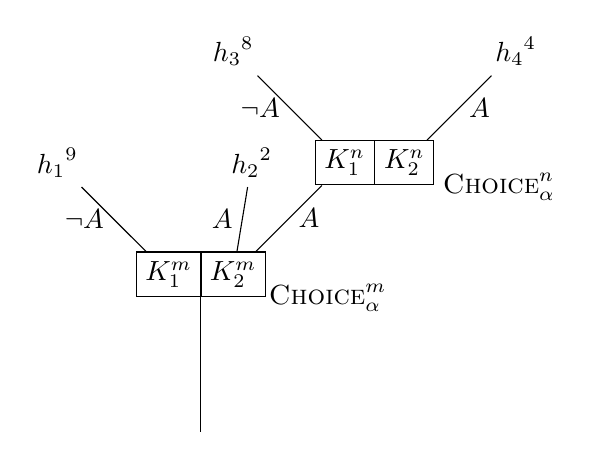
\begin{tikzpicture}[node distance=2cm]
        \node (start) {};
        \node[draw,rectangle] (choice11) [above of=start] {$K_1^m$};
        \node[draw,rectangle] (choice12) [right of=choice11,xshift=-1.18cm] {$K_2^m$};
        \node (choicem) [right of=choice12,yshift=-0.3cm,xshift=-0.8cm] {$\textsc{Choice}_\alpha^m$};
        \node (h1) [above left of=choice11] {${h_1}^9$};
        \node (h2) [above right of=choice12,xshift=-1.18cm] {${h_2}^2$};
        \node[draw,rectangle] (choice21) [above right of=choice12] {$K_1^n$};
        \node[draw,rectangle] (choice22) [right of=choice21,xshift=-1.24cm] {$K_2^n$};
        \node (choicen) [right of=choice22,yshift=-0.3cm,xshift=-0.8cm] {$\textsc{Choice}_\alpha^n$};
        \node (h3) [above left of=choice21] {${h_3}^8$};
        \node (h4) [above right of=choice22] {${h_4}^4$};
        
        \draw
        ([xshift=.4cm]start.center) edge ([xshift=.4cm]choice11.center)
        (choice12) edge node[left] {$A$} (h2)
        (choice12) edge node[right] {$A$} (choice21)
        (choice21) edge node[left] {$\lnot A$} (h3)
        (choice22) edge node[right] {$A$} (h4)
        (choice11) edge node[left] {$\lnot A$} (h1);
    \end{tikzpicture}
    \caption{An example of a STIT-tree}
    \label{fig:stit-tree}
\end{figure}

In these trees the interior nodes -- in our case $\textsc{Choice}^m_{\alpha}$ and $\textsc{Choice}^n_{\alpha}$ -- are moments in time where a decision can be made by the agent in question. In this context a decision at moment $m$ is a set of actions, of which the agent must take exactly one. For $\textsc{Choice}^m_{\alpha}$ the agent $\alpha$ can decide between $K_1^m$ and $K_2^m$, so $\textsc{Choice}^m_{\alpha} = \{K_1^m, K_2^m\}$. Actions can be non-deterministic, i.e. the same action may lead to multiple different outcomes -- this is the case for $K_2^m$.

Depending on which action the agent takes, he either will be presented with another decision or reach an outcome. The leafs in those trees are the histories or traces of made decisions, and with each of them is associated a utility value that is based on the state reached, e.g. $h_1$ has a utility of $9$. Finally, each edge is assigned a set of propositions that are true at this point in time.

\subsection{Semantic on STIT-trees}
For the semantics we always look at a moment-history pair $m, h$ and check whether $m,h\models \varphi$ holds. If our formula is simply an atomic proposition $A$, we get $m,h\models A$ iff $A$ is true at the outgoing edge of $m$ on the path to $h$. For example, this is the case for $m,h_3$ but not for $m, h_1$ and $n,h_3$. A formula $\mathcal{F} A$ is fulfilled iff $A$ holds at some point on the path from $m$ to $h$ (e.g. $m,h_3\models \mathcal{F} A$ but also $m,h_3\models \mathcal{F} \neg A$). The relation $m,h\models \bigcirc A$ holds iff $A$ holds on all edges of $m$ that reach histories having the highest utility value for those histories reachable from $m$. Note how $h$ is irrelevant. For example, this is the case for $m,h_2\models \bigcirc A$ since $A$ holds in the best history reachable from $m$, namely, $h_4$. 

To deal not only with obligations but also agents, we introduce a new operator: $[\alpha \cstit \colon A]$ meaning that $\alpha$ sees to it that $A$ (\emph{stit} for \emph{sees to it that} and the \emph{c} from the name of the logician \emph{Chellas}). The relation $m,h\models [\alpha \cstit \colon A]$ is fulfilled iff $A$ is true for every pair $m, h'$ that belongs to the same action as $m,h$. This is the case for $m,h_3$ since $A$ holds at every outgoing edge of $K^m_2$.


\section{Non-deterministic actions and the gambling problem}
In order to reapply the known deontic logic semantics in the world of agent systems, one may intuitively think that the obligation to do something is the same as the obligation that something will be done or that a certain history will be reached. This, however, becomes challenging if an action may lead to multiple histories in an unpredictable manner. 

\subsection{The gambling problem}
The first problem concerning agents the authors talk about is the \emph{gambling problem} \cite{mdl}. In this scenario an agent is presented with two options -- he gambles and either doubles or loses his bet or he does not gamble and thus preserves his money. An example tree for which the agent starts with 5€ is given in Figure~\ref{fig:gambling-tree}. Here the utility value describes how much money he has in the end and the proposition $G$ means \enquote{he gambles}. The question is whether he should gamble hoping for the sweet win but also risking to lose everything or rather refrain from doing so.

\begin{figure}[ht]
    \centering
     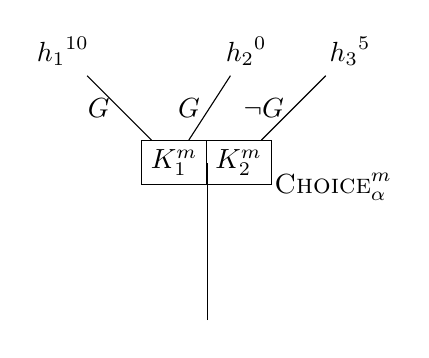
\begin{tikzpicture}[node distance=2cm]
        \node (start) {};
        \node[draw,rectangle] (choice11) [above of=start] {$K_1^m$};
        \node[draw,rectangle] (choice12) [right of=choice11,xshift=-1.18cm] {$K_2^m$};
        \node (choicem) [right of=choice12,yshift=-0.3cm,xshift=-0.8cm] {$\textsc{Choice}_\alpha^m$};
        \node (h1) [above left of=choice11] {${h_1}^{10}$};
        \node (h2) [above right of=choice11, xshift=-.5cm] {${h_2}^0$};
        \node (h3) [above right of=choice12] {${h_3}^5$};
        
        \draw
        ([xshift=.42cm]start.center) edge ([xshift=.42cm]choice11.center)
        (choice11) edge node[left] {$G$} (h1)
        (choice11) edge node[left] {$G$} (h2)
        (choice12) edge node[left] {$\neg G$} (h3);
    \end{tikzpicture}
    \caption{An example STIT-tree for the gambling problem}
    \label{fig:gambling-tree}
\end{figure}

\subsection{Optimality of non-deterministic actions}
The optimal path would end in $h_1$, so in order to get to this best outcome the agent should \enquote{ought to see to it that G}. Intuitively, one would try to formalize this with $\bigcirc[\alpha \cstit \colon G]$, however, the action $K^m_1$ is not necessarily the better option because, in the end, the outcome of the gamble comes down to luck. 

This problem arises from the fact that we define the optimality of a history only by its utility value disregarding that the actions that lead to this history are non-deterministic. Or in other words, while an optimal history concerns ought-to-be and optimal actions concern ought-to-do, we cannot infer the optimal action from the optimal history because an action may lead non-deterministically to multiple (and potentially worse) histories. Rather, we should correspond actions to sets of histories and compare the optimality of all possible histories to determine the optimal action.

Horty suggested that an action $K_1$ should be considered more optimal than $K_2$ if each of its histories have at least the same utility value than any of the histories reachable from $K_2$, while the other way is not the case. This leads to a new operator $\odot [\alpha \cstit \colon G]$ meaning \enquote{$\alpha$ ought to see to it that $G$}. This formula is fulfilled iff for each action not leading to $G$ there is a better action that does lead to $G$. Since $K_1^m$ and $K_2^m$ correspond to equally good sets of histories, neither $\odot [\alpha \cstit \colon G]$ nor $\odot [\alpha \cstit \colon \neg G]$ hold for $m$.


\section{Moral Luck}
In some cases the utility of an agents decision might be dependent on another agents decision. This becomes particularly problematic if this dependence is circular and the involved agents have no way of communicating or reasoning about the decisions of the others.

\subsection{The driving problem}
In \cite{mdl} the authors discuss this problem with the example of the \emph{driving problem}:

Suppose an agent $\alpha$ is driving on a small road and another driver, agent $\beta$, is travelling towards $\alpha$. Both agents have the option of swerving to the side or continuing to drive straight. However, should they decide on the same action they will collide. It's obvious that there are two good and two bad outcomes: the good ones are, where only one of the persons moves to the side, the bad ones are where both move to the side or both don't move. 
Figure~\ref{fig:driving-problem} illustrates how $\alpha$ has to decide between $K_1^m$(swerve) and $K_2^m$(do not swerve) and $\beta$ between $K_3^m$(swerve) and $K_4^m$(do not swerve). Depending on the combination of their decisions $m$ either leads to an optimal solution $h_1$ or $h_3$ or they crash in $h_2$ or $h_4$. The proposition $S$ stands for \enquote{$\alpha$ swerves}.

\begin{figure}[ht]
    \centering
     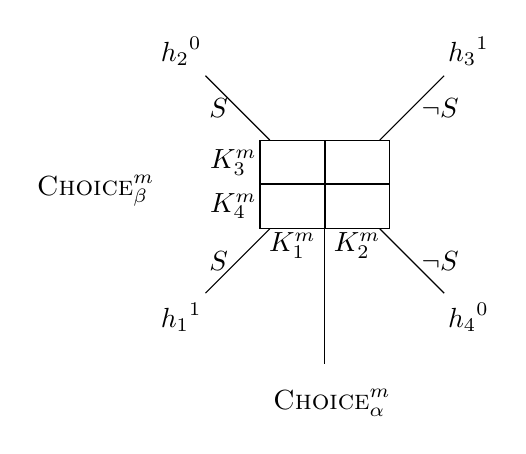
\begin{tikzpicture}[node distance=2cm]
        \node (start) {};
        \node[draw,rectangle, text opacity=0] (choice11) [above of=start] {$K_1^m$};
        \node (K1) [below of=choice11, yshift=1.5cm] {$K_1^m$};
        \node[draw,rectangle, text opacity=0] (choice12) [right of=choice11,xshift=-1.18cm] {$K_2^m$};
        \node (K2) [below of=choice12, yshift=1.5cm] {$K_2^m$};
        \node[draw,rectangle, text opacity=0] (choice13) [above of=choice11,yshift=-1.45cm] {$K_3^m$};
        \node (K3) [left of=choice13, xshift=1.25cm] {$K_3^m$};
        \node[draw,rectangle, text opacity=0] (choice14) [right of=choice13,xshift=-1.18cm] {$K_4^m$};
        \node (K4) [left of=choice11, xshift=1.25cm] {$K_4^m$};
        
        \node (choicem) [below of=start, yshift=1.5cm, xshift=.5cm] {$\textsc{Choice}_\alpha^m$};
        \node (choicen) [left of=choice11, yshift=.2cm, xshift=-.5cm] {$\textsc{Choice}_\beta^m$};
        \node (h1) [below left of=choice11] {${h_1}^1$};
        \node (h2) [above left of=choice13] {${h_2}^0$};
        \node (h3) [above right of=choice14] {${h_3}^1$};
        \node (h4) [below right of=choice12] {${h_4}^0$};
        
        \draw
        ([xshift=.41cm]start.center) edge ([xshift=.41cm]choice11.center)
        (choice11) edge node[left] {$S$} (h1)
        (choice12) edge node[right] {$\neg S$} (h4)
        (choice13) edge node[left] {$S$} (h2)
        (choice14) edge node[right] {$\neg S$} (h3);
    \end{tikzpicture}
    \caption{A STIT-tree for the driving problem}
    \label{fig:driving-problem}
\end{figure}

This problem is somewhat similar to the gambling problem since the utility of an action of an agent is based on external influences. In this case, however, it is not a random event, but the action of another independent agent whose actions $\alpha$ cannot reason about. 

\subsection{Dominance act utilitarianism and orthodox perspective}
We now face the problem whether $\odot [\alpha \cstit \colon S]$ should be true or not at the moment of the decision. There are generally two established views on this problem.

The first is dominance act utilitarianism, where an action is only optimal, if each of its outcomes is optimal. More formally the formula $\odot [\alpha \cstit \colon S]$ is true only if all actions that lead to optimal outcomes also guarantee $S$. Since this is not the case in the driving problem, we have that $\odot [\alpha \cstit \colon S]$ does not hold at moment $m$. Note that this is also the case for $\odot [\alpha \cstit \colon \lnot S]$ since both actions (swerving and staying in lane) may lead to optimal outcomes, which agent $\alpha$ ought to strive for.

In the second view, the orthodox perspective, we also take into consideration the actual circumstances the agent will find themselves in after making the decision. Intuitively $\alpha$ should ask themselves what \emph{would} the best decision have been. This means that instead of looking at $\odot [\alpha \cstit \colon S]$, we can answer the question of whether $\bigcirc [\alpha \cstit \colon S]$ should be true at moment $m$ for the history $h$ that occurred. In this case $\bigcirc [\alpha \cstit \colon S]$ is true for $h_1$ and $h_4$, and likewise $\bigcirc [\alpha \cstit \colon \lnot S]$ is true for $h_2$ and $h_3$.

\section{Procrastination}
Another problem that arises is the problem of procrastination. If an agent agrees to take on an obligation, the agent may indefinitely put off following through with that obligation until a deadline is reached. This is especially a problem if the highest utility is achieved by that specific agent taking on that obligation and then following through.

\subsection{Professor Procrastinate}
The example given in \cite{mdl} describes a professor -- aptly named Professor Procrastinate -- who is asked to write a review. As he is the best person available for this, the optimal situation is him agreeing to write the review and then actually doing it. However, this professor is known to procrastinate and even though he has the choice to actually write the review, he will not in fact do that, thus the review will never be written. Since this is the worst case it would be better for him to decline the request so that someone else can write the review.

This leads us to the contradiction that the professor ought to accept the request and write the review since this is the optimal course of action, but at the same time he ought to decline the request since doing otherwise will lead to the worst possible outcome.

\subsection{Fields and actualism}
The problem that leads to the contradiction is the existence of a possible choice that is in a way already settled. A possible solution to this problem is to narrow down the choices we will take into consideration to those that are actual choices. This view on the problem is fittingly named actualism.

For a STIT-tree this means we will only consider a subset of the possible choices, which gives us a sub-tree of the problem that may be a more appropriate model of reality. We call this sub-tree, on which we will evaluate a formula, a \emph{field}.

For the example of Professor Procrastinate we can safely take into consideration only the first choice as him accepting or declining the request will not change the fact that he will not write the review. So our field will contain only the first decision. Since we are now no longer allowed to reason about the possibility of the professor writing the review, it is easy to see that he ought to decline.

Let us take a look at what this means for the semantics of the formula $\odot [\pi \cstit \colon A]$, where $\pi$ is the professor and $A$ is the decision to accept the request. If our field contains all possible choices -- a view which is also called \emph{possibilism} -- then $\odot [\pi \cstit \colon A]$ should be true, since this is the only choice leading to the optimal outcome. But using the field containing only the first choice we have that $\odot [\pi \cstit \colon A]$ is false, since with the background assumption that Professor Procrastinate will not write the review, the actual optimal outcome can only be reached if the professor declines.

\section{Summary}
Despite seeming like a straightforward conclusion to talk about actions by talking about histories inferred by them, it is not as simple as to reduce \emph{ought-to-do} to \emph{ought-to-be-done}. Rather, one has to accommodate for the specifics that come with the usage of agency, including, among other things, different histories caused by non-deterministic actions, multiple agents influencing each other and the difference between what \emph{could} happen and what \emph{actually} happens.


\bibliographystyle{IEEEbib}
\nocite{*}
\bibliography{refs}

\end{document}
